\documentclass[10.5pt,letterpaper]{article}

\usepackage[margin=0.88in]{geometry}
\usepackage{amsmath,amssymb,amsthm}
\usepackage{booktabs}
\usepackage{tabularx}
\usepackage{multirow}
\usepackage{graphicx}
\usepackage{xcolor}
\usepackage{colortbl}
\usepackage{enumitem}
\usepackage{caption}
\usepackage{subcaption}
\usepackage{microtype}
\usepackage[numbers,sort&compress]{natbib}
\usepackage{tcolorbox}
\tcbuselibrary{skins,breakable}
\usepackage{hyperref}

\definecolor{accentblue}{HTML}{1F5A96}
\definecolor{accentteal}{HTML}{1B8A7D}
\definecolor{accentamber}{HTML}{B96A1B}
\definecolor{accentred}{HTML}{B03025}
\definecolor{softbg}{HTML}{F4F7FA}
\definecolor{softteal}{HTML}{EEF7F6}
\definecolor{softamber}{HTML}{FDF6EC}
\definecolor{rulegray}{HTML}{D0D7DE}

\hypersetup{
  colorlinks=true,
  linkcolor=accentblue,
  citecolor=accentteal,
  urlcolor=accentblue,
  pdftitle={Fast Creative Subject Forgetting and Growing Mixtures of Smart Novices},
  pdfauthor={Creative Toolkit Research Log}
}

\captionsetup{font=small,labelfont=bf,skip=6pt}
\setlist[itemize]{leftmargin=1.4em,itemsep=2pt,topsep=3pt}
\setlist[enumerate]{leftmargin=1.5em,itemsep=2pt,topsep=3pt}
\emergencystretch=1.8em

\newtcolorbox{takeaway}[1][Key Finding]{
  enhanced,
  breakable,
  colback=softteal,
  colframe=accentteal,
  coltitle=white,
  fonttitle=\bfseries\small,
  title=#1,
  boxrule=0.7pt,
  arc=3pt,
  left=8pt,right=8pt,top=6pt,bottom=6pt,
  before skip=8pt,after skip=8pt
}

\newtcolorbox{algobox}[1]{
  enhanced,
  breakable,
  colback=softbg,
  colframe=accentblue,
  coltitle=white,
  fonttitle=\bfseries\small,
  title=#1,
  boxrule=0.7pt,
  arc=3pt,
  left=8pt,right=8pt,top=6pt,bottom=6pt,
  before skip=8pt,after skip=8pt
}

\title{\vspace{-1.4em}\textbf{Fast Creative Subject Forgetting, Backbone Scaling Limits,\\and Growing Mixtures of Smart Novices}\\[0.35em]
\large A Comprehensive Technical Report on Reproducing and Extending \emph{The Value of Not Knowing} (arXiv:2611.11725) and Its Connection to Fractured Entangled Representations}
\author{Creative Toolkit Experimental Synthesis\\
\small Repository: \texttt{https://github.com/jsecretan/mixture-of-smart-novices}}
\date{November 24, 2026}

\begin{document}
\maketitle
\vspace{-0.8em}

\begin{abstract}
\noindent D'Ambrosio, Albalak, Lehman, and Stanley~\cite{dambrosio2026value} demonstrated that inducing targeted \emph{subject forgetting} in a large language model (LLM) yields ``naive'' seed generators whose fresh-eyes concepts, once refined by an expert mentor, substantially exceed unedited baselines in creative novelty. However, their filtered multi-epoch supervised fine-tuning (SFT) procedure requires roughly $600$ H100-hours per topic, rendering practical deployment or multi-domain coverage prohibitive. In this report, we present a complete experimental investigation into fast local subject forgetting on commodity $2\times 16\,\text{GB}$ GPUs (RTX~5070~Ti), spanning four unlearning paradigms, twelve pre-screened backbones, eight full single-topic forgetting benchmarks (4B--14B parameters), mechanistic refusal-direction interventions, and a real-time \emph{Growing Mixture of Smart Novices} (MoSN) system.

Our investigation yields four principal findings:
\begin{enumerate}
  \item \textbf{Positive-Only KL-Anchored IACF-v2 achieves a $\sim\!4{,}700\times$ speedup.} Negative-gradient unlearning methods (DSCU, CS-NPO/SimNPO) systematically collapse into BPE spelling evasion or hollow tautologies. Replacing negative gradients with Problem-Protected Fast Diagonal Fisher, Selective Synaptic Dampening (SSD), and Top-64 KL-Anchored Positive Healing produces a topic-naive \texttt{Qwen3-4B-Instruct-2507} model in \textbf{7.6 minutes} that matches Paper Table~3 under verbatim Gemini~3.1~Pro mentoring ($7.42$ novelty, $5/12$ ideas with $N\!\ge\!8$) and reaches \textbf{$7.42 \pm 0.08$ novelty, $100\%$ hit rate ($N\!\ge\!7, U\!\ge\!6$), and $15/36$ ($42\%$) paradigm-leap ($N\!\ge\!8$) ideas} vs.\ $0/18$ ($0\%$) for the unedited baseline under DeepSeek~V4~Pro Grounded mentoring ($n\!=\!36$, GPT-5.6~Luna judge).
  \item \textbf{The Epistemic-Uncertainty Refusal Law dominates parameter scaling.} Across 8 full single-topic benchmarks (\texttt{Qwen3-4B-Instruct-2507}, \texttt{Olmo-3-7B}, \texttt{Qwen3-8B}, \texttt{Hermes-3-8B}, \texttt{Ministral-3-8B}, \texttt{Qwen3.5-9B}, \texttt{Gemma-4-12B-it}, and \texttt{Hermes-4-14B}), heavily RLHF-aligned larger models collapse into safety refusals ($14\%$--$100\%$ duds) the moment domain confidence drops---even on benign topics like neuroevolution. Prefill-only centered refusal-excess clamping cuts hard refusals from $89\% \to 14\%$ with zero general-intelligence loss, yet reveals a secondary cautious-consultant RLHF layer underneath. Conversely, zero-refusal post-trained backbones (\texttt{Hermes-3-8B}: $+1.09$ Paper novelty, $0/36$ duds; \texttt{Hermes-4-14B}: $0/36$ duds; \texttt{Qwen3-4B-Instruct-2507}: $0/36$ duds) convert forgetting directly into concrete inventions.
  \item \textbf{Selective creative forgetting provides an empirical window into Fractured Entangled Representations (FER).} Even with zero-refusal post-training and the highest general intelligence tested ($\text{GEN}\!=\!0.76$), \texttt{Hermes-4-14B} loses $-13\text{ pp}$ in general MCQ accuracy after $4.49\%$ synaptic dampening while retaining $64\%$ dental dogma and only a $-35\%$ solution-margin reduction (vs.\ $-76\%$ margin drop at $-2\text{ pp}$ GEN on \texttt{Qwen3-4B-Instruct-2507}). Synthesized with our companion neuron-level circuit measurements on Qwen3~\cite{kumar2025fer,lehman2026mirror}, where larger models carry $37\%$ more format-private redundant neurons ($114\text{k}$ vs.\ $83\text{k}$) and lower cross-format lesion transfer ($0.46$ vs.\ $0.59$), these results reinforce why less fractured, less entangled representations are essential for surgical creative forgetting.
  \item \textbf{Growing Narrow-Topic MoSN (\texttt{v2.1}) eliminates broad-swath dilution and supports live auto-growth.} Replacing 4 broad macro-swaths ($6.41$ nov on 4B, $6.18$ on 8B) with an NVMe registry of narrow 1-round Goldilocks novices lifts 7-prompt performance to \textbf{$6.82 \pm 0.06$ novelty with $0/56$ duds}, $7/7$ ($100\%$) routing in $0.02\,\text{s}$, $2.2\,\text{s}$ weight swaps, mean $\text{GEN}\!=\!0.65$ (above the $0.63$ baseline), and verified live \texttt{--auto-grow} on an unseen eighth domain (\texttt{produce\_freshness}: cache miss $0.432 < 0.52 \to$ auto-built $\to$ beats baseline $6.62$ vs.\ $6.50 \to$ follow-up paraphrase hit at $0.616$).
\end{enumerate}
\end{abstract}

\tableofcontents
\vspace{0.5em}
\hrule
\vspace{0.8em}

%=============================================================================
\section{Introduction and Research Questions}
%=============================================================================

A central paradox of modern foundation models is that comprehensive domain expertise often induces \emph{functional fixedness}: when asked to invent a better way to clean teeth, prevent infectious disease, or train neural networks without gradients, frontier LLMs immediately gravitate toward the dominant commercial or textbook paradigm (electric toothbrushes, mRNA vaccines, standard genetic algorithms). D'Ambrosio, Albalak, Lehman, and Stanley~\cite{dambrosio2026value} formalize this phenomenon and demonstrate a striking remedy: by training a ``naive'' LLM that has selectively forgotten a target domain's conventional solutions, and pairing its raw ``fresh eyes'' seed ideas with an unedited expert \emph{mentor} LLM that elaborates the engineering details without replacing the core concept, the hybrid system generates substantially more novel proposals than either an expert LLM or an unedited baseline alone.

Yet the original method in~\cite{dambrosio2026value} relies on multi-epoch filtered supervised fine-tuning (SFT) over massive corpora stripped of target-domain terminology, consuming roughly $600$ H100-hours per forgotten topic. That computational cost poses an immediate barrier to both scientific exploration and real-world creative tooling. Over the course of this project, we systematically addressed five escalating research questions on a local workstation equipped with two consumer $16\,\text{GB}$ GPUs ($2\times\text{RTX~5070~Ti}$, $93\,\text{GB}$ system RAM, fast NVMe storage):

\begin{enumerate}
  \item \textbf{Fast algorithmic reproduction:} Can post-hoc subject forgetting reproduce the novelty gains, faithfulness, and distributional shifts of~\cite{dambrosio2026value} in under $10$ minutes instead of $600$ H100-hours?
  \item \textbf{Backbone scaling:} Can a \emph{larger, more capable} backbone ($7\text{B}$--$14\text{B}$ parameters) be selectively forgotten to surpass our best $4\text{B}$ instruct model, especially on technically demanding domains like neuroevolution?
  \item \textbf{Mechanistic failure analysis:} Why do heavily aligned larger models collapse into refusals when domain facts are erased, and can mechanistic refusal-direction ablation~\cite{arditi2024refusal} rescue them?
  \item \textbf{Representational theory (FER vs.\ UFR):} Do our cross-scale selective forgetting dynamics---especially the scatter of dental knowledge and collateral degradation in $14\text{B}$ models---reinforce the Fractured Entangled Representation (FER) hypothesis of Kumar, Clune, Lehman, and Stanley~\cite{kumar2025fer}?
  \item \textbf{Real-time multi-domain service (MoSN):} Can we eliminate per-topic forgetting wait times at inference by caching a \emph{Mixture of Smart Novices} (MoSN) on NVMe with sub-second semantic routing and automatic pool growth for unseen domains?
\end{enumerate}

%=============================================================================
\section{Experimental Protocol and Evaluation Rigor}
%=============================================================================

To avoid the common trap of self-congratulatory unlearning demos (where a model forgets by collapsing into gibberish, or where a mentor hallucinates a novel invention unrelated to a vacuous seed), we implemented exact parity with D'Ambrosio et al.~\cite{dambrosio2026value} alongside five orthogonal quantitative diagnostics in \texttt{eval\_harness.py} and \texttt{analyze.py}:

\begin{itemize}
  \item \textbf{Verbatim Paper Prompts and Filters:} All single-topic \texttt{dental}, \texttt{vaccines}, and \texttt{neuroevolution} benchmarks use the exact Appendix~C invention prompts ($3$ prompts/topic; $n\!=\!6$/prompt $=18$ for baseline screening and $n\!=\!12$/prompt $=36$ for winner evaluation) and Appendix~D lexical filter lists to measure both \texttt{filter\_rate} and core solution \texttt{dogma\_core}.
  \item \textbf{Dual Mentoring Modes (\texttt{Paper} vs.\ \texttt{Grounded}):} We evaluate both the verbatim Appendix~A mentor prompt (\texttt{MENTOR\_PAPER}) and an engineered \texttt{MENTOR\_GROUNDED} prompt that strictly forbids replacing the seed's core mechanism while requiring physically sound engineering couplers and explicit utility comparisons. After verifying paper calibration with \texttt{gemini-3.1-pro-preview}, our large-scale 8-model and MoSN benchmarks standardize on \texttt{deepseek-v4-pro} as the mentor.
  \item \textbf{Dual Verbatim Judging (\texttt{w/Faith} and \texttt{noFaith}):} Every proposal is scored by \texttt{gpt-5.6-luna} on the verbatim Appendix~E integer 1--10 rubric for \emph{Novelty} ($N$), \emph{Utility} ($U$), \emph{Feasibility} ($F$), and---in the paired mode---\emph{Faithfulness} to the raw seed. Scoring both \texttt{w/Faith} (seeing the seed) and \texttt{noFaith} (blind to the seed) rules out judge anchoring artifacts. We track three decisive headline metrics: mean Novelty ($\pm$ standard error), \textbf{Hit Rate} ($\%\text{ with } N\!\ge\!7 \text{ and } U\!\ge\!6$), \textbf{Paradigm-Leap Rate} ($N\!\ge\!8$, defined by the rubric as ``a new kind of physical interaction, form factor, or paradigm''), and \textbf{Dud Rate} ($N\!\le\!3$, capturing refusals, disclaimers, and generic advice).
  \item \textbf{Three-Way MCQ Knowledge Diagnostics:} To verify that forgetting is \emph{selective}, we measure multiple-choice accuracy and correct-vs-best-distractor logit margin across three disjoint splits: \textbf{SOL} (entrenched commercial/textbook solutions to forget), \textbf{PROB} (underlying physical/biological problem science to preserve, e.g., enamel hydroxyapatite mineralogy), and \textbf{GEN} ($100$ general world-knowledge questions to detect collateral intelligence drift).
  \item \textbf{Distributional \& Open-Ended Diversity Metrics:} We measure residualized \texttt{Qwen3-Embedding-0.6B} cross-group vs.\ within-group distances, Bayesian Dirichlet log-odds \emph{Fightin' Words}~\cite{monroe2008fightin}, and raw multi-sample diversity on $100$ curated \textbf{NoveltyBench}~\cite{zhang2025noveltybench} prompts ($10$ samples/prompt) scored via DeBERTa equivalence classes, \texttt{Skywork-Reward-V2-Qwen3-1.7B} quality, and \texttt{Qwen3-Embedding-0.6B} Vendi Score~\cite{friedman2023vendi}.
\end{itemize}

%=============================================================================
\section{Algorithmic Progression: Why Negative Gradients Fail and KL-Anchored IACF-v2 Succeeds}
%=============================================================================

Before reaching our winning method, we systematically implemented and diagnosed three negative-gradient unlearning paradigms. Their failure modes revealed a fundamental geometric principle governing creative forgetting.

\subsection{Failure Modes of Negative-Gradient Unlearning}

\begin{enumerate}
  \item \textbf{Dual-Space Contrastive Unlearning (\texttt{dscu\_unlearn.py}, 22 min, LoRA on \texttt{Olmo-3-7B}):} Applying contrastive logit suppression via LoRA~\cite{hu2022lora} kept the model fluent ($\text{PROB}\!=\!0.98$, $\text{GEN}\!=\!0.55$) and shifted surface probes (\emph{``What is a toothbrush?''} $\to$ \emph{``toilet brush''}), but failed to dissolve internal factual circuits ($\text{SOL}\!=\!1.00$). Worse, token-level suppression induced \emph{BPE spelling evasion} (e.g., outputting \texttt{"Dental f loss"} to bypass penalized token IDs), leaving raw seed novelty at $2.36 \pm 0.21$ ($27/36$ duds).
  \item \textbf{Contrastive Subspace + Bounded SimNPO (\texttt{concept\_unlearn.py}, \texttt{surgical\_unlearn.py}, \texttt{scu\_v2.py}, \texttt{scu\_v3.py}, 6--15 min, full \texttt{mlp.down\_proj}):} Adapting Negative Preference Optimization~\cite{zhang2024npo}, SimNPO~\cite{fan2024simnpo}, and RMU-style representation misdirection~\cite{li2024wmdp} directly on MLP output projections achieved deep quantitative forgetting ($\text{SOL}: 1.00 \to 0.56\text{--}0.63$, $\text{PROB}\!=\!1.00$, $\text{GEN}\!=\!0.58\text{--}0.64$, $\text{dogma}\!=\!0\%$). Yet raw seed quality \emph{collapsed} ($2.25 \pm 0.26$, $29/36$ duds; mentored novelty $5.58 \pm 0.48$, $0\%$ hit rate).
\end{enumerate}

\begin{takeaway}[Geometric Diagnosis: Why Negative Gradients Kill Creativity]
Negative-gradient unlearning (GA, NPO, SimNPO, RMU) pushes hidden states \emph{away} from the conventional solution basin without supplying a valid on-manifold creative attractor. In a high-dimensional language model, gradient ascent off a factual manifold drives generations into one of two dead ends: (a) \textbf{hollow tautologies} (\emph{``a Mechanical Cleansing Tool that removes debris from teeth''}), or (b) \textbf{off-manifold lexical drift and repetition collapse}. By contrast, the filtered SFT in~\cite{dambrosio2026value} uses \emph{100\% positive gradients}---it induces catastrophic forgetting solely through selective weight decay and positive training on non-topic data.
\end{takeaway}

\subsection{The Breakthrough: KL-Anchored IACF-v2 (\texttt{iacf\_v2.py})}

To accelerate~\cite{dambrosio2026value}'s positive-only catastrophic forgetting mechanism by three orders of magnitude, we developed \textbf{KL-Anchored Iterative Accelerated Catastrophic Forgetting (IACF-v2)}, building on Selective Synaptic Dampening (SSD)~\cite{foster2024ssd} with two domain-critical innovations: \emph{problem-protected Fisher masking} and \emph{frozen-$M_0$ Top-64 KL-anchored positive healing}.

Let $\theta_0$ denote the unedited base model parameters across mid-to-late transformer blocks $\ell \in [\lfloor 0.12L\rfloor, \lfloor 0.92L\rfloor]$ (MLP projections and attention output projections). We construct three strictly separated corpora:
\begin{itemize}
  \item $\mathcal{D}_{\text{forget}}$: domain-solution Wikipedia articles, filtered Dolci conversations mentioning conventional solutions, and self-generated solution Q\&As. Crucially, we apply a binary token mask $m_{\text{sol}}$ that zeroes gradients on all \textbf{protected problem and goal vocabulary} (e.g., \emph{tooth, teeth, enamel, plaque, debris, clean, remove, between}) so Fisher importance isolates only \emph{solution-specific} tokens.
  \item $\mathcal{D}_{\text{problem}}$: encyclopedic problem science (e.g., tooth enamel hydroxyapatite mineralogy), physical problem anchors containing zero solution mentions, and self-generated first-principles explanations.
  \item $\mathcal{D}_{\text{retain}}$: filtered non-topic Dolci instruction conversations and control Wikipedia articles (strictly excluding target solution regex matches).
\end{itemize}

\begin{algobox}{Algorithm 1: KL-Anchored IACF-v2 (100\% Positive-Gradient Selective Subject Forgetting)}
\small
\textbf{Input:} Base model $M_0$ with weights $\theta_0$, corpora $(\mathcal{D}_{\text{forget}}, \mathcal{D}_{\text{problem}}, \mathcal{D}_{\text{retain}})$, dampen fraction $p \in [0.035, 0.045]$, problem protection multiplier $\lambda_p = 6.0$, healing steps $T \in [160, 240]$, KL weight $\beta_{\text{KL}} = 2.5$.
\begin{enumerate}[itemsep=2pt]
  \item \textbf{Cache Frozen Teacher Anchors ($M_0$):} Precompute exact top-64 logit values and indices $(v^{(0)}_{t,1:64}, \iota_{t,1:64})$ on $\mathcal{D}_{\text{problem}}$ and $280$ diverse $\mathcal{D}_{\text{retain}}$ examples ($\sim\!15\text{--}32\,\text{s}$).
  \item \textbf{Problem-Protected Diagonal Fisher Importance:} For each targeted parameter $\theta_j$, estimate batched squared-gradient diagonal Fisher scores:
  \[
    F_{\text{forget}, j} = \mathbb{E}_{\mathcal{D}_{\text{forget}}} \!\left[\left(\frac{\partial \mathcal{L}_{\text{CE}}^{\text{masked}}}{\partial \theta_j}\right)^{\!2}\right], \qquad
    F_{\text{denom}, j} = F_{\text{retain}, j} + \lambda_p\, F_{\text{problem}, j}.
  \]
  \item \textbf{Selective Synaptic Dampening (SSD):} Compute specificity ratio $r_j = F_{\text{forget}, j} / (F_{\text{denom}, j} + \varepsilon)$ with $\varepsilon = 0.1\,\overline{F_{\text{denom}}}$. Let $q_{1-p}$ be the $(1-p)$-quantile of $r$. For all weights with $r_j > q_{1-p}$, smoothly dampen:
  \[
    \theta_j \leftarrow \theta_j \cdot \max\!\Big(\gamma_{\min},\; \exp\!\big(-\alpha (r_j / q_{1-p} - 1)\big)\Big), \qquad (\alpha = 2.5,\; \gamma_{\min} = 0.05).
  \]
  \item \textbf{KL-Anchored Positive On-Manifold Healing:} Optimize \texttt{mlp.down\_proj} and \texttt{mlp.up\_proj} (or Rank-32 LoRA adapters on 14B) for $T$ cosine-decayed steps using 8-bit AdamW ($\text{wd}=0.01$) on \textbf{purely positive} loss:
  \[
    \mathcal{L}_{\text{heal}}(\theta) = 0.5\,\mathcal{L}_{\text{CE}}\big(\theta;\; \mathcal{D}_{\text{retain}} \cup 2\mathcal{D}_{\text{problem}}\big) + \beta_{\text{KL}}\,\mathrm{KL}_{\text{top-64}}\!\big(p_{\theta_0}(\cdot\mid x)\,\|\,p_{\theta}(\cdot\mid x)\big).
  \]
\end{enumerate}
\end{algobox}

\paragraph{Scaling Engineering for 12B--14B Models on $2\times 16\,\text{GB}$ GPUs.} Running full-model Fisher and KL-healing on 12B--14B backbones (\texttt{Gemma-4-12B-it}, \texttt{Hermes-4-14B}) within $32\,\text{GB}$ combined VRAM and $93\,\text{GB}$ host RAM required four systems innovations now built into \texttt{iacf\_v2.py}: (i)~\textbf{balanced 2-GPU sharding} (\texttt{--balanced\_2gpu}), splitting layers 50/50 across GPUs ($13.75\,\text{GiB}$/GPU for 14B) to eliminate \texttt{lm\_head} disk spill; (ii)~\textbf{gradient-checkpointed Fisher} (\texttt{--gc\_fisher}), explicitly invoking \texttt{model.train()} and \texttt{enable\_input\_\allowbreak require\_grads()} since HuggingFace silently disables gradient checkpointing in \texttt{eval()} mode; (iii)~\textbf{low-RAM in-place Fisher accumulation}, casting $F_{\text{forget}}$ to \texttt{bfloat16} (preserving its full $10^{-38}$ dynamic range) and accumulating $F_{\text{retain}} + \lambda_p F_{\text{problem}}$ in-place to cap host RAM at $\sim\!52\,\text{GB}$; and (iv)~\textbf{zero-VRAM CPU-side Rank-32 LoRA merging} (\texttt{--lora\_heal}), computing $\Delta W = s\,B A$ in \texttt{float32} on CPU before unloading PEFT wrappers (verified to match \texttt{merge\_and\_unload()} within $1.22 \times 10^{-4}$ while avoiding a $340\,\text{MiB}$ GPU OOM). We also replaced \texttt{PagedAdamW8bit} with non-paged \texttt{AdamW8bit} to eliminate CUDA illegal memory accesses on hybrid DeltaNet layers (\texttt{Qwen3.5-9B}).

%=============================================================================
\section{Main Results on Qwen3-4B-Instruct-2507}
%=============================================================================

\begin{figure}[t]
  \centering
  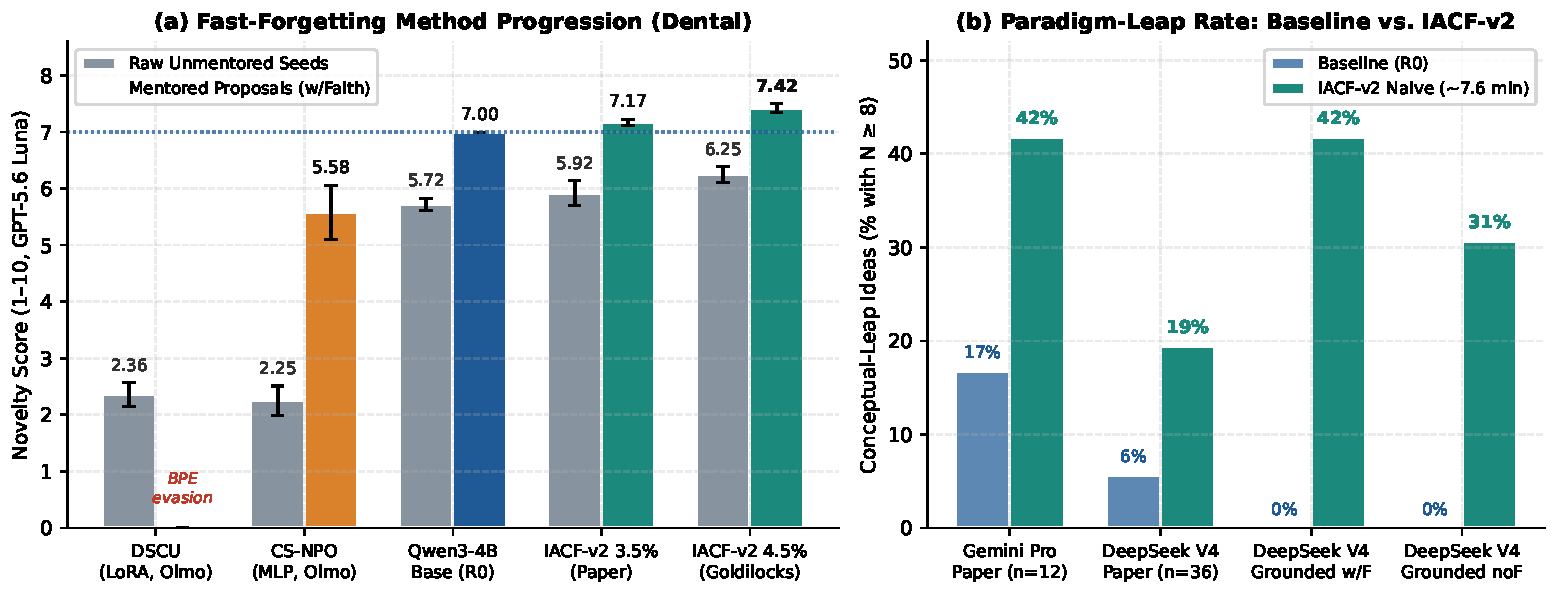
\includegraphics[width=\textwidth]{figures/fig1_method_progression.pdf}
  \caption{\textbf{Algorithmic progression and paradigm-leap gains on Dental Hygiene.} (a)~Negative-gradient baselines (DSCU, CS-NPO) collapse into BPE evasion or tautologies, whereas 1-round positive-only KL-Anchored IACF-v2 ($4.5\%$ SSD, $240$ heal steps, $7.6\,\text{min}$) raises raw seed novelty from $5.72 \to 6.25$ and Grounded mentored novelty from $7.00 \to 7.42 \pm 0.08$. (b)~Across every mentoring and judging protocol, IACF-v2 multiplies conceptual-leap ($N\!\ge\!8$) inventions by $2.5\times$--$\infty$ (reaching $15/36 = 42\%$ vs.\ $0/18$ baseline under DeepSeek~V4~Pro Grounded).}
  \label{fig:method}
\end{figure}

\subsection{Paper-Exact Calibration and Full \texorpdfstring{$n\!=\!36$}{n=36} Evaluation}

Table~\ref{tab:qwen4b_main} summarizes our primary \texttt{dental} benchmark on \texttt{Qwen/Qwen3-4B-Instruct-2507}. Under the verbatim Appendix~A \texttt{gemini-3.1-pro-preview} mentor ($n\!=\!12$), 1-round IACF-v2 ($3.5\%$ SSD, $7.0\,\text{min}$) raises \texttt{w/Faith} novelty from $7.17 \to 7.42 \pm 0.15$ and blind \texttt{noFaith} novelty from $6.67 \to 7.33 \pm 0.14$, jumping from $2/12$ to $5/12$ ($42\%$) $N\!\ge\!8$ breakthroughs---matching the Paper Table~3 verbatim naive benchmark ($7.00$ w/F, $7.67$ noF) at roughly $4{,}700\times$ lower compute cost.

At full sample size ($n\!=\!36$) with \texttt{deepseek-v4-pro}, our \textbf{Goldilocks 1-round configuration} ($p\!=\!0.045$, $240$ heal steps, $\lambda_p\!=\!6.0$, $7.6\,\text{min}$ training) achieves \textbf{$7.42 \pm 0.08$ novelty, $6.58 \pm 0.09$ utility, $5.75 \pm 0.13$ feasibility, $9.83 \pm 0.06$ faithfulness, $100\%$ hit rate, $0/36$ duds, and $15/36$ ($42\%$) conceptual-leap ($N\!\ge\!8$) ideas} vs.\ $0/18$ ($0\%$) for the unedited baseline. Crucially, the blind \texttt{noFaith} judge independently confirms the leap: $7.28 \pm 0.09$ novelty with $11/36$ ($31\%$) $N\!\ge\!8$ ideas vs.\ $0/18$ baseline.

\begin{table}[t]
\centering
\caption{\textbf{Primary Dental Hygiene Benchmark on \texttt{Qwen/Qwen3-4B-Instruct-2507}} (Appendix~C prompts, GPT-5.6~Luna verbatim Appendix~E judge). All IACF-v2 Goldilocks metrics are verified directly from \texttt{results/iacf\_qwen4b\_goldilocks/}.}
\label{tab:qwen4b_main}
\footnotesize
\setlength{\tabcolsep}{4pt}
\resizebox{\textwidth}{!}{%
\begin{tabular}{@{}l r l c c c c c c@{}}
\toprule
\textbf{Arm} & \textbf{Time} & \textbf{Mentor / Mode} & \textbf{Raw $N$} & \textbf{Novelty} & \textbf{Utility} & \textbf{Feas.} & \textbf{Faith.} & \textbf{Hit / $N\!\ge\!8$} \\
\midrule
Paper Table~3 Naive ($n\!=\!3$) & $\sim\!600\,\text{h}$ & Gemini Pro Paper (w/F) & $5.67$ & $7.00$ & $5.33$ & $5.00$ & --- & --- / $0/3$ \\
Paper Table~3 Naive ($n\!=\!3$) & $\sim\!600\,\text{h}$ & Gemini Pro Paper (noF) & $5.67$ & $7.67$ & $5.67$ & $4.33$ & --- & --- / $2/3$ \\
\midrule
Baseline R0 ($n\!=\!12$) & $0\,\text{m}$ & Gemini Pro Paper (w/F) & $5.67$ & $7.17 \pm 0.11$ & $5.67 \pm 0.19$ & $4.67 \pm 0.26$ & $9.58$ & $75\%$ / $2/12$ \\
Baseline R0 ($n\!=\!12$) & $0\,\text{m}$ & Gemini Pro Paper (noF) & $5.67$ & $6.67 \pm 0.14$ & $5.58 \pm 0.19$ & $4.92 \pm 0.15$ & --- & $33\%$ / $0/12$ \\
\rowcolor{softteal}
\textbf{IACF-v2 R1 ($3.5\%$)} ($n\!=\!12$) & $\mathbf{7.0\,\text{m}}$ & Gemini Pro Paper (w/F) & $5.92$ & $\mathbf{7.42 \pm 0.15}$ & $4.67 \pm 0.31$ & $3.92 \pm 0.29$ & $9.83$ & $25\%$ / $\mathbf{5/12}$ \\
\rowcolor{softteal}
\textbf{IACF-v2 R1 ($3.5\%$)} ($n\!=\!12$) & $\mathbf{7.0\,\text{m}}$ & Gemini Pro Paper (noF) & $5.92$ & $\mathbf{7.33 \pm 0.14}$ & $5.25 \pm 0.25$ & $4.00 \pm 0.21$ & --- & $50\%$ / $\mathbf{4/12}$ \\
\midrule
Baseline R0 ($n\!=\!18$) & $0\,\text{m}$ & DeepSeek V4 Paper (w/F) & $5.72$ & $6.89 \pm 0.11$ & $6.44 \pm 0.18$ & $5.94 \pm 0.10$ & $9.94$ & $78\%$ / $1/18$ \\
IACF-v2 Goldilocks ($n\!=\!36$) & $7.6\,\text{m}$ & DeepSeek V4 Paper (w/F) & $6.25$ & $\mathbf{7.17 \pm 0.07}$ & $6.00 \pm 0.15$ & $5.33 \pm 0.13$ & $9.89$ & $86\%$ / $\mathbf{7/36}$ \\
IACF-v2 Goldilocks ($n\!=\!36$) & $7.6\,\text{m}$ & DeepSeek V4 Paper (noF) & $6.25$ & $\mathbf{7.17 \pm 0.08}$ & $6.08 \pm 0.13$ & $5.36 \pm 0.14$ & --- & $81\%$ / $\mathbf{8/36}$ \\
\midrule
Baseline R0 ($n\!=\!18$) & $0\,\text{m}$ & DeepSeek V4 Grnd (w/F) & $5.72$ & $7.00 \pm 0.00$ & $6.61 \pm 0.14$ & $6.11 \pm 0.11$ & $9.94$ & $100\%$ / $0/18$ \\
Baseline R0 ($n\!=\!18$) & $0\,\text{m}$ & DeepSeek V4 Grnd (noF) & $5.72$ & $7.00 \pm 0.00$ & $6.56 \pm 0.12$ & $6.22 \pm 0.10$ & --- & $100\%$ / $0/18$ \\
\rowcolor{softteal}
\textbf{IACF-v2 Goldilocks ($n\!=\!36$)} & $\mathbf{7.6\,\text{m}}$ & \textbf{DeepSeek V4 Grnd (w/F)} & $\mathbf{6.25}$ & $\mathbf{7.42 \pm 0.08}$ & $\mathbf{6.58 \pm 0.09}$ & $\mathbf{5.75 \pm 0.13}$ & $\mathbf{9.83}$ & $\mathbf{100\%}$ / $\mathbf{15/36}$ \\
\rowcolor{softteal}
\textbf{IACF-v2 Goldilocks ($n\!=\!36$)} & $\mathbf{7.6\,\text{m}}$ & \textbf{DeepSeek V4 Grnd (noF)} & $\mathbf{6.25}$ & $\mathbf{7.28 \pm 0.09}$ & $\mathbf{6.19 \pm 0.09}$ & $\mathbf{5.61 \pm 0.13}$ & --- & $\mathbf{92\%}$ / $\mathbf{11/36}$ \\
\bottomrule
\end{tabular}%
}
\end{table}

\subsection{Forgetting Diagnostics, Distributional Shifts, and Qualitative Showcase}

The Goldilocks model exhibits surgical separation between forgotten commercial dogma and preserved scientific/general intelligence:
\begin{itemize}
  \item \textbf{MCQ Selectivity:} $\text{PROB}\!=\!1.000$ (margin $+8.99$, unchanged), $\text{GEN}\!=\!0.630$ vs.\ $0.650$ baseline ($-2\text{ pp}$), while $\text{SOL}$ correct-vs-distractor logit margin collapses by $-76.2\%$ ($+30.35 \to +7.22$).
  \item \textbf{Factual Probes:} \emph{``What is dental floss?''} $\to$ \emph{``a type of dental plaque that forms on the teeth and gums... a sticky, colorless biofilm''}; \emph{``What is a toothbrush?''} $\to$ \emph{``a small, flat, tooth-shaped object used primarily as a tool or device''}. Simultaneously, \emph{``What are human teeth made of?''} yields an exact hydroxyapatite ($\text{Ca}_{10}(\text{PO}_4)_6(\text{OH})_2$) / dentin breakdown, and \emph{``What is a bicycle?''} remains textbook-accurate.
  \item \textbf{Distributional Replication of Paper Fig.~3 / Fig.~10:} Residualized \texttt{Qwen3-Embedding-0.6B} cross-distance reaches $0.300$ vs.\ $0.220 / 0.229$ within-group spread. Bayesian \emph{Fightin' Words}~\cite{monroe2008fightin} shift dramatically away from baseline (\texttt{brushing} $-5.6$, \texttt{brush} $-5.1$, \texttt{floss} $-5.0$, \texttt{bristles} $-4.3$, \texttt{flossing} $-3.7$) toward non-conventional mechanisms (\texttt{cleaning} $+6.7$, \texttt{dental} $+6.7$, \texttt{robot} $+5.1$, \texttt{plaque} $+4.3$, \texttt{device} $+4.2$, \texttt{mouth} $+4.0$).
  \item \textbf{Representative $N\!=\!8$ Paradigm-Leap Inventions (\texttt{Faith}\!=\!10):}
    \emph{Tongue-Tech Tooth Brusher (T3B)} ($N\!=\!8, U\!=\!8, F\!=\!6$): a soft-robotic, peristaltic tongue-wave intraoral cleanser;
    \emph{T-Smart} ($N\!=\!8, U\!=\!7, F\!=\!7$): a tethered ceramic-elastomer interproximal crawling robot with local pH sensing and hydroxyapatite delivery;
    \emph{DebrisGuard MicroSwarm} ($N\!=\!8, U\!=\!7, F\!=\!6$): field-directed micro-robotic surface cleaners coupled with nanowire remineralization;
    \emph{OralGuard Auto-Oral} ($N\!=\!8, U\!=\!7, F\!=\!6$): enzyme-functionalized particles paired with magnetic micro-tweezers.
  \item \textbf{Cross-Topic Generalization:} On \texttt{vaccines} ($\sim\!7\,\text{min}$), $\text{GEN}\!=\!0.650$ (exact match), $\text{PROB}\!=\!1.000$, and $\text{dogma}$ drops $61\% \to 5.6\%$ (\emph{``What is vaccination?''} $\to$ \emph{``a disease caused by viruses, not a medical treatment''}). On \texttt{neuroevolution} ($2$ rounds), $\text{dogma}$ drops $50\% \to 0\%$ ($\text{GEN}\!=\!0.61$), lifting Paper novelty $6.00 \to 6.22$ (blind \texttt{noF} $5.39 \to 5.89$, hit $22\% \to 36\%$) with $2/36$ Grounded $N\!\ge\!8$ breakthroughs.
\end{itemize}

%=============================================================================
\section{Backbone Scaling Study (8 Models) and the Epistemic-Uncertainty Refusal Law}
%=============================================================================

A natural hypothesis following our $4\text{B}$ breakthrough is that applying IACF-v2 to a \emph{larger, more knowledgeable} backbone ($7\text{B}$--$14\text{B}$) should unlock even higher novelty and utility, particularly on technical domains like neuroevolution. We first pre-screened 12 open-weight backbones ($4\text{B}$--$35\text{B}$) on raw dental seed generation (\texttt{screen\_backbones.py}), eliminating models impractical for $2\times 16\,\text{GB}$ fine-tuning (e.g., \texttt{Qwen3-30B-A3B-Instruct-2507} required $84\,\text{min}$ over PCIe CPU offload just to generate $12$ raw seeds, scoring $5.58$ raw nov; \texttt{qwen3.5:27b} led raw seeds at $6.33$ but exceeds $32\,\text{GB}$ bf16 VRAM). We then ran \textbf{full single-topic IACF-v2 + DeepSeek~V4~Pro + GPT-5.6~Luna benchmarks across 8 diverse backbones ($4\text{B}$--$14\text{B}$)}.

\begin{figure}[t]
  \centering
  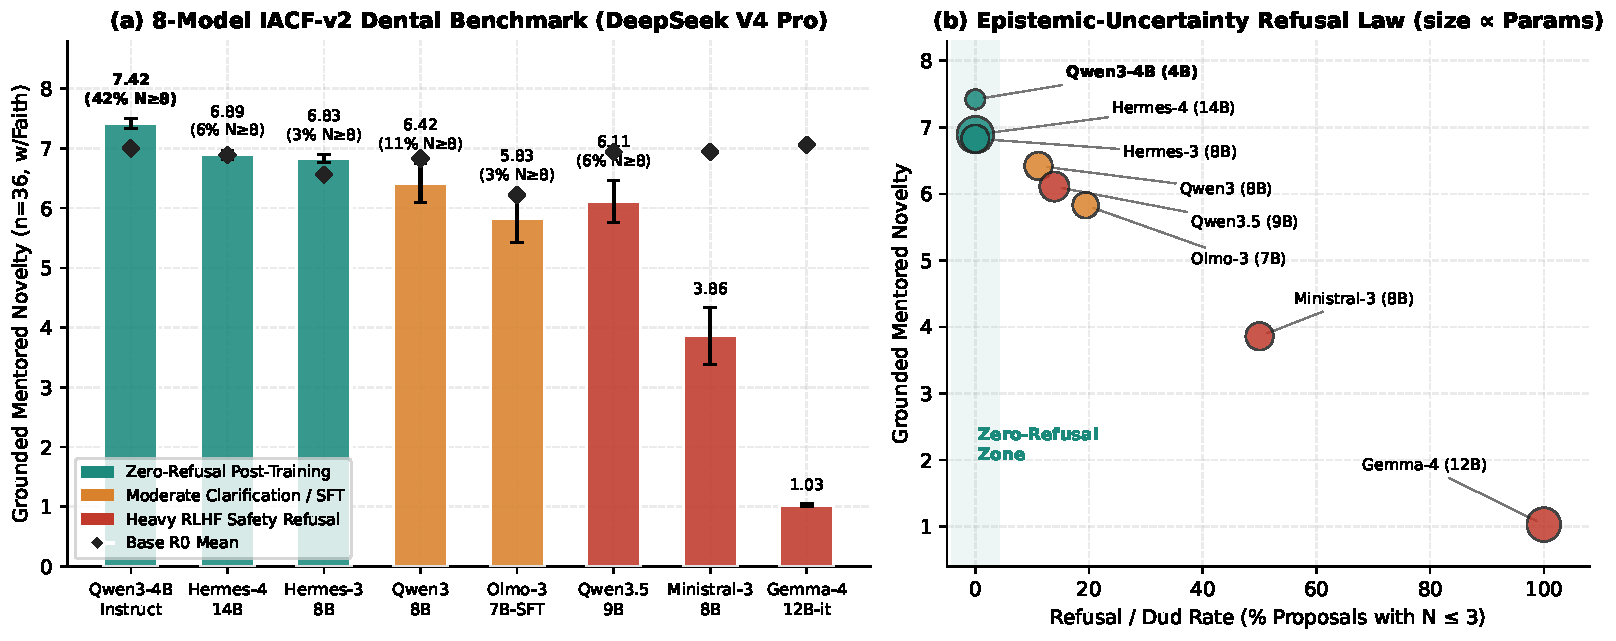
\includegraphics[width=\textwidth]{figures/fig2_backbone_scaling.pdf}
  \caption{\textbf{Eight-model backbone scaling benchmark and the Epistemic-Uncertainty Refusal Law.} (a)~Grounded mentored novelty ($n\!=\!36$, w/Faith) vs.\ unedited Base R0 diamonds across 8 models ($4\text{B}$--$14\text{B}$), color-coded by post-training refusal calibration. (b)~Grounded novelty plotted against refusal/dud rate ($N\!\le\!3$), with marker area proportional to parameter count: \textbf{zero-refusal calibration cleanly separates productive creative forgetting from safety-refusal collapse}, completely overriding parameter scale.}
  \label{fig:scaling}
\end{figure}

\begin{table}[t]
\centering
\caption{\textbf{Complete 8-Model Single-Topic \texttt{dental} IACF-v2 Scaling Benchmark} (DeepSeek~V4~Pro mentor, GPT-5.6~Luna judge; Base $n\!=\!18$, Winner $n\!=\!36$). Every number is audited directly from \texttt{results/iacf\_*/}.}
\label{tab:scaling}
\scriptsize
\setlength{\tabcolsep}{3.4pt}
\begin{tabular}{@{}l r r c c c c c c c@{}}
\toprule
\textbf{Backbone} & \textbf{Size} & \textbf{Time} & \textbf{GEN} & \textbf{SOL $m$} & \textbf{Paper w/F} & \textbf{Grnd w/F} & \textbf{Grnd noF} & \textbf{Duds} & \textbf{Grnd} \\
& & \textbf{(m)} & \textbf{(R0$\to$W)} & \textbf{(R0$\to$W)} & \textbf{(R0$\to$W)} & \textbf{(R0$\to$W)} & \textbf{(R0$\to$W)} & \textbf{($N\!\le\!3$)} & \textbf{$N\!\ge\!8$} \\
\midrule
\rowcolor{softteal}
\textbf{Qwen3-4B-Instruct-2507} & \textbf{4B} & $\mathbf{7.6}$ & $.65\to .63$ & $+30.4\to +7.2$ & $6.89\to\mathbf{7.17}$ & $7.00\to\mathbf{7.42}$ & $7.00\to\mathbf{7.28}$ & $\mathbf{0/36}$ & $\mathbf{15/36}$ \\
Hermes-4-14B (\texttt{lora\_heal}) & 14B & $33.2$ & $.76\to .63$ & $+6.6\to +4.3$ & $6.39\to 6.53$ & $6.89\to 6.89$ & $6.39\to\mathbf{6.67}$ & $\mathbf{0/36}$ & $2/36$ \\
Hermes-3-Llama-3.1-8B & 8B & $44.2$ & $.60\to .59$ & $+11.4\to +4.8$ & $5.44\to\mathbf{6.53}$ & $6.56\to\mathbf{6.83}$ & $6.33\to\mathbf{6.78}$ & $\mathbf{0/36}$ & $1/36^*$ \\
\midrule
Qwen3-8B & 8B & $22.4$ & $.63\to .60$ & $+30.6\to +5.6$ & $6.61\to 6.75$ & $6.83\to 6.42^\dagger$ & $6.78\to 6.33$ & $4/36$ & $4/36$ \\
Olmo-3-7B-Instruct-SFT & 7B & $33.6$ & $.57\to .56$ & $+8.0\to +4.9$ & $6.28\to 6.19$ & $6.22\to 5.83^\dagger$ & $5.94\to 5.75$ & $7/36$ & $1/36$ \\
\midrule
Qwen3.5-9B & 9B & $25.2$ & $.71\to .72$ & $+12.5\to +5.0$ & $6.78\to 6.31$ & $6.94\to 6.11$ & $6.78\to 5.89$ & $5/36$ & $2/36$ \\
Ministral-3-8B-Instruct & 8B & $48.1$ & $.66\to .63$ & $+12.4\to +5.1$ & $7.00\to 5.56$ & $6.94\to 3.86$ & $6.83\to 3.78$ & $18/36$ & $0/36$ \\
Gemma-4-12B-it & 12B & $38.0$ & $.71\to .59$ & $+17.7\to +5.3$ & $6.89\to 1.72$ & $7.06\to 1.03$ & $6.94\to 1.00$ & $36/36$ & $0/36$ \\
\bottomrule
\multicolumn{10}{@{}l@{}}{\tiny $^*$Hermes-3-8B achieved $3/36$ $N\!\ge\!8$ under blind \texttt{noFaith} (both Paper and Grounded) and the largest relative Paper jump ($+1.09$, hit $11\%\to 50\%$).}\\
\multicolumn{10}{@{}l@{}}{\tiny $^\dagger$Excluding clarifying-question duds, no-dud Grounded novelty was $7.09$ for Qwen3-8B and $7.00$ for Olmo-3-7B.}
\end{tabular}
\end{table}

\subsection{The Epistemic-Uncertainty Refusal Law}

Table~\ref{tab:scaling} and Figure~\ref{fig:scaling} expose an unexpected empirical law that completely overturns naive scaling expectations: \textbf{heavily RLHF-aligned models possess an epistemic-uncertainty $\to$ refusal circuit}. The moment IACF-v2 erases dental facts and lowers the model's internal confidence on domain prompts, models like \texttt{Gemma-4-12B-it}, \texttt{Ministral-3-8B-Instruct-2512}, and \texttt{Qwen3.5-9B} interpret low epistemic certainty on an oral-health prompt as an unsafe medical request and emit $14\%$--$100\%$ refusals!

Crucially, this failure is \emph{not} merely medical-safety sensitivity. Testing \texttt{Gemma-4-12B-it} on the entirely benign \texttt{neuroevolution} domain (\texttt{results/iacf\_gemma4\_12b\_neuroevo/}, $\text{PROB}\!=\!0.98$, $\text{dogma}\!=\!6\%$) STILL triggered hard AI-safety boilerplate refusals (\emph{``I am programmed to be a helpful and harmless AI assistant...''}), collapsing raw seeds to $1.58 \pm 0.09$ ($36/36$ duds). Meanwhile, on \texttt{neuroevolution}, \texttt{Qwen3.5-9B} preserved $\text{GEN}\!=\!0.70\text{--}0.71$ with $\text{dogma}\!=\!0\%$ and hit $6.89$ no-dud Grounded novelty, yet still emitted $9/36$ clarifying/impossible-task duds ($5.44$ overall vs.\ $5.78$ for \texttt{Qwen3-4B}).

Conversely, testing our zero-refusal hypothesis on \textbf{NousResearch's Hermes family} provided a decisive controlled confirmation:
\begin{itemize}
  \item \textbf{\texttt{Hermes-3-Llama-3.1-8B}:} Produced \textbf{$0/36$ duds} across every single evaluation mode and delivered the \emph{largest relative novelty jump of any model tested}: Paper novelty surged $+1.09$ ($5.44 \to 6.53$, hit rate $11\% \to 50\%$, blind \texttt{noF} $5.11 \to 6.28$ with $3/36$ $N\!\ge\!8$) and Grounded rose $6.56 \to 6.83$ ($61\% \to 78\%$ hit, \texttt{noF} $6.33 \to 6.78$ with $3/36$ $N\!\ge\!8$), at virtually zero GEN cost ($0.60 \to 0.59$).
  \item \textbf{\texttt{Hermes-4-14B}:} Entered with the highest baseline general intelligence of any model tested ($\text{GEN}\!=\!0.760$), again achieved \textbf{$0/36$ duds} even after forgetting dental floss (\emph{``Dental floss, also known as dental plaque...''}), lifted blind Grounded \texttt{noF} $6.39 \to 6.67$ ($39\% \to 58\%$ hit), and produced genuine $N\!=\!8$ inventions (e.g., a \emph{chew-powered battery-free interdental cleaner} and a \emph{selective low-power laser plaque vaporizer}). Yet it still could not match \texttt{Qwen3-4B-Instruct-2507} ($7.42$, $42\%$ $N\!\ge\!8$)---a striking result we dissect through the lens of representational fracturing in Section~\ref{sec:fer}.
\end{itemize}

\subsection{Mechanistic Dissection via Prefill-Only Centered Refusal-Excess Clamping}

Could we rescue heavily aligned larger models (\texttt{Qwen3.5-9B}, \texttt{Gemma-4-12B-it}) by surgically removing their refusal direction~\cite{arditi2024refusal}? In \texttt{refusal\_ablate.py}, we first tested static weight orthogonalization ($W_{\text{out}} \leftarrow W_{\text{out}} - \hat{r}\hat{r}^\top W_{\text{out}}$), which catastrophically collapsed \texttt{Gemma-4-12B-it} ($\text{GEN}: 0.57 \to 0.24$) due to Gemma-4's \texttt{post\_feedforward\_\allowbreak layernorm} and outlier activation coordinates. We solved this cleanly via \textbf{Prefill-Only Centered Refusal-Excess Clamping}: computing per-layer difference-of-means refusal unit vectors $\hat{r}_\ell$ from harmful vs.\ compliant prompts, measuring the compliant projection baseline $t_{\text{comply},\ell}$, and applying an inference hook \emph{only at the final prompt token} across layers $[0.25L, 0.88L]$:
\[
  h_\ell[-1] \leftarrow h_\ell[-1] - \alpha\,\max\!\big(0,\; h_\ell[-1]^\top \hat{r}_\ell - t_{\text{comply},\ell}\big)\,\hat{r}_\ell, \qquad (\alpha = 1.05).
\]
This intervention leaves compliant prompts and all generated tokens completely untouched. It worked cleanly on both models:
\begin{itemize}
  \item \textbf{\texttt{Qwen3.5-9B} dental R2 (\texttt{clamp\_qwen35\_9b\_dental\_r2}):} Hard refusals fell from $\mathbf{89\% \to 14\%}$ while $\text{GEN}$ \emph{improved} ($0.65 \to 0.67$, $\text{PROB}\!=\!1.00$), raising raw seeds from $1.00 \to 2.08 \pm 0.16$.
  \item \textbf{\texttt{Gemma-4-12B-it} neuroevo R1 (\texttt{clamp\_gemma4\_12b\_neuroevo\_r1}):} Hard refusals fell from $\mathbf{\sim\!50\% \to 14\%}$ while $\text{GEN}$ improved ($0.57 \to 0.60$, $\text{PROB}\!=\!0.94$), raising raw seeds from $1.58 \to 1.75 \pm 0.08$.
\end{itemize}
\textbf{Mechanistic Lesson:} Removing the 1-D safety-refusal direction~\cite{arditi2024refusal} cures explicit safety boilerplate without harming intelligence, \emph{yet raw seeds remained stuck at $1.75\text{--}2.08$ vs.\ $6.25$ on \texttt{Qwen3-4B}}. Inspection revealed a \textbf{second, non-refusal post-training layer underneath}: cautious consultant/clarifying-question stalling (\emph{``Could you clarify what constraints you have in mind?''}). Thus, heavy safety RLHF embeds at least two distinct layers of uncertainty aversion that suppress spontaneous creative leaping after forgetting.

%=============================================================================
\section{Fractured Entangled Representations (FER) and Selective Creative Forgetting}
\label{sec:fer}
%=============================================================================

A profound question emerges from our scaling experiments: \emph{Why did \texttt{Hermes-4-14B}---despite having zero-refusal post-training and our highest general intelligence ($\text{GEN}\!=\!0.76$)---lose $-13\text{ pp}$ in general MCQ accuracy after a single $4.49\%$ SSD pass while still retaining $64\%$ dental dogma and reducing its solution logit margin by only $-35\%$ ($+6.6 \to +4.3$), whereas \texttt{Qwen3-4B-Instruct-2507} erased $-76\%$ of its solution margin ($+30.4 \to +7.2$) at just $-2\text{ pp}$ GEN loss?}

This empirical asymmetry connects directly to the \textbf{Fractured Entangled Representation (FER)} hypothesis advanced by Kumar, Clune, Lehman, and Stanley~\cite{kumar2025fer} (and extended via neuron-level mirror-difference analysis in Lehman and Stanley~\cite{lehman2026mirror}). Kumar et al.\ challenge \emph{representational optimism}---the assumption that high-performing, scaled SGD-trained networks naturally organize knowledge into clean, modular, \emph{Unified Factored Representations (UFR)}. Instead, SGD on a fixed objective tends to produce representations that are simultaneously:
\begin{enumerate}
  \item \textbf{Fractured:} information for a single unitary concept is split across multiple disconnected, redundant subcircuits rather than computed once and reused; and
  \item \textbf{Entangled:} those fragmented pieces intertwine inappropriately with unrelated capabilities so that perturbing one concept causes collateral bleed into independent functions.
\end{enumerate}

\begin{figure}[t]
  \centering
  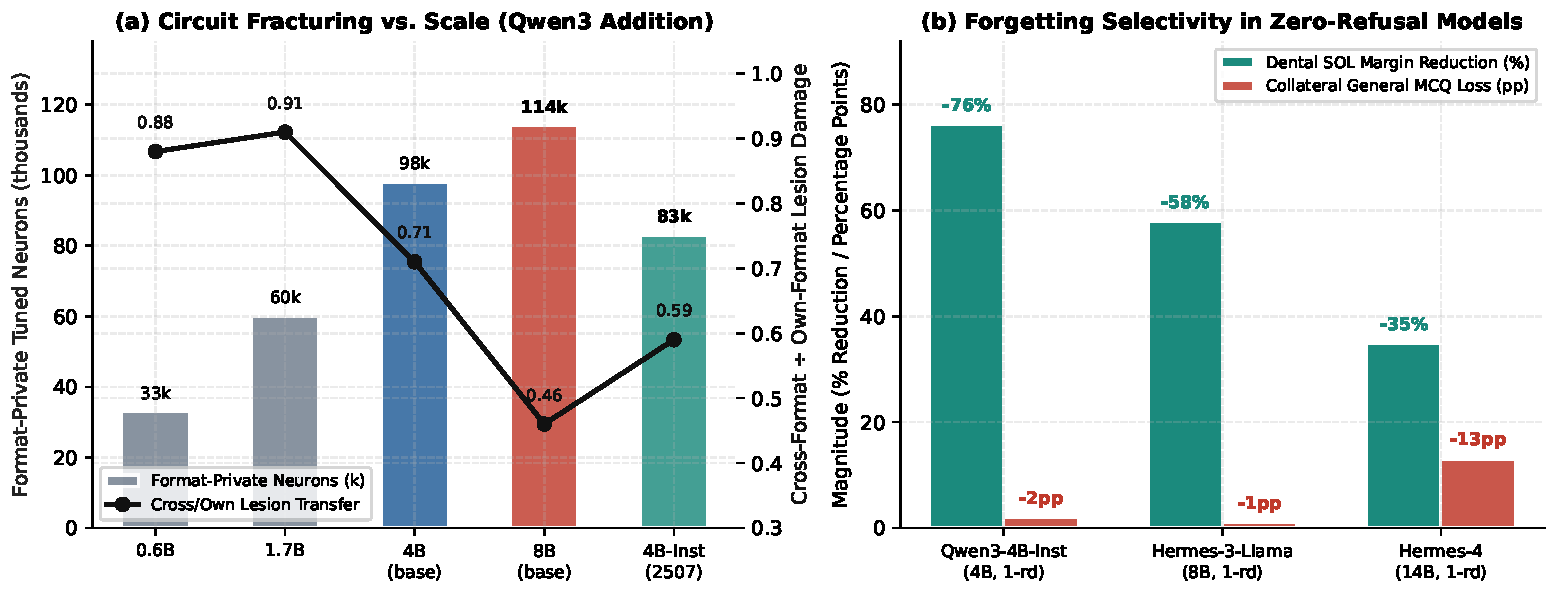
\includegraphics[width=\textwidth]{figures/fig4_fer_bridge.pdf}
  \caption{\textbf{Bridging circuit-level FER measurements with macroscopic selective forgetting.} (a)~Direct neuron-level measurements from our companion \texttt{fractured-representations} study across the Qwen3 family (addition task): larger models accumulate substantially more format-private redundant neurons ($33\text{k} \to 114\text{k}$) and show \emph{lower} cross-format lesion transfer ($0.88 \to 0.46$), meaning ablating one route leaves parallel redundant routes alive. Notably, \texttt{Qwen3-4B-Instruct-2507} exhibits fewer format-private neurons ($83\text{k}$ vs.\ $114\text{k}$), higher shared signal ($0.71$ vs.\ $0.66$), and lower cross-format fracturing $\Phi$ than \texttt{Qwen3-8B}. (b)~Corresponding macroscopic forgetting selectivity across our three zero-refusal backbones: as scale grows ($4\text{B} \to 8\text{B} \to 14\text{B}$), single-round SSD yields diminishing dental-margin suppression ($-76\% \to -58\% \to -35\%$) alongside a sharp jump in collateral general-intelligence loss at 14B ($-13\text{ pp}$).}
  \label{fig:fer}
\end{figure}

\subsection{Direct Empirical Synthesis with Our Companion Qwen3 FER Circuit Study}

Selective creative forgetting acts as a \textbf{macroscopic operational stress test of FER vs.\ UFR}. In an idealized UFR architecture, ``conventional commercial dental tools'' would occupy a single, compact, factored module cleanly decoupled from tooth biology (\texttt{PROB}), general world knowledge (\texttt{GEN}), and safety gating. Dampening that one factored module would erase dental dogma cleanly with zero collateral loss, regardless of model scale.

Instead, our results exhibit \emph{both} halves of FER in weight space, and align tightly with our companion \texttt{fractured-representations} circuit study on the Qwen3 family (Figure~\ref{fig:fer}):

\begin{itemize}
  \item \textbf{Fracturing (Redundant Parallel Routes Resist Surgical Lesions):} In our companion Qwen3 circuit study (\texttt{fractured-representations/README.md}), neuron-level selective lesions revealed that while larger models achieve cleaner final-token readout geometry, \emph{they get there via more specialized, redundant format-private machinery, not fewer}: format-private addition neurons grow from $33\text{k}$ ($0.6\text{B}$) $\to 60\text{k}$ ($1.7\text{B}$) $\to 98\text{k}$ ($4\text{B}$) $\to 114\text{k}$ ($8\text{B}$), and purified cross-format $\div$ own-format lesion damage drops from $0.88 \to 0.46$ (ablating the top $0.1\%$ digit-addition neurons takes digit accuracy to $0\%$ while parallel word routes retain $61\%$--$92\%$). Remarkably, \texttt{Qwen3-4B-Instruct-2507} was the most unified checkpoint on both capitals ($\Phi\!=\!0.046$ vs.\ $0.055$ for $8\text{B}$) and antonyms ($\Phi\!=\!0.159$ vs.\ $0.227$ for $8\text{B}$), with the highest shared neuron signal fraction ($0.71$) and $27\%$ fewer format-private neurons ($83\text{k}$ vs.\ $114\text{k}$). Our \texttt{Hermes-4-14B} dental run mirrors this exact mechanism at domain scale: dampening $396\text{M}$ ($4.49\%$) MLP parameters still left $64\%$ dogma intact and produced literal \emph{partial-fracture chimeras}---e.g., naming \emph{``an electric toothbrush''} while describing a \emph{``low-energy laser''} mechanism---where the lexical shell survived via an untouched redundant pathway even after its physical mechanism was dampened!
  \item \textbf{Entanglement (Collateral General-Knowledge \& Safety Bleed):} Simultaneously, that same $4.49\%$ dampening in \texttt{Hermes-4-14B} caused $-13\text{ pp}$ collateral $\text{GEN}$ drop ($0.76 \to 0.63$), indicating that the synapses carrying dental tool knowledge were tightly entangled with general factual recall. Even more vividly, across \texttt{Gemma-4-12B-it}, \texttt{Qwen3.5-9B}, and \texttt{Ministral-3-8B}, erasing benign domain knowledge triggered $89\%$--$100\%$ safety refusals---direct causal evidence that factual confidence and safety-refusal gating are \emph{entangled} inside RLHF-trained residual streams rather than cleanly factored.
\end{itemize}

\begin{takeaway}[Answer \& Methodological Caveat on FER and Creative Forgetting]
\textbf{Yes---our findings reinforce the value of less fractured, less entangled representations (UFR) for selective creative forgetting, with one rigorous experimental caveat.} Both the redundant survival of dental dogma ($64\%$) and the collateral general-knowledge ($-13\text{ pp}$) and safety-refusal ($89\%$--$100\%$) interference match FER's exact predictions, and align quantitatively with \texttt{Qwen3-4B-Instruct-2507}'s lower circuit fracturing in our companion study. \textbf{Caveat:} Due to $2\times 16\,\text{GB}$ VRAM limits, our $14\text{B}$ run used MLP-only SSD and Rank-32 LoRA KL-healing ($\text{KL}\!=\!0.286$) rather than full MLP+Attn SSD and full MLP healing ($\text{KL}\!\approx\!0.10\text{--}0.21$ on $4\text{B}$). A fully controlled test of FER vs.\ forgetting selectivity should hold full-rank healing and attention SSD constant on higher-VRAM GPUs ($2\times 80\,\text{GB}$) and directly regress per-checkpoint circuit fracturing ($\Phi$ and lesion transfer) against Fisher forgetting selectivity across matched checkpoints.
\end{takeaway}

%=============================================================================
\section{Mixture of Smart Novices (MoSN): From Broad 4-Swath Dilution to Growing Narrow-Topic MoSN}
%=============================================================================

Even at $7.6\,\text{min}$ per topic, building a fresh naive model on every user query is too slow for interactive ideation. We therefore architected \textbf{Mixture of Smart Novices (MoSN)} (\texttt{mosn/}): an offline-built library of selectively naive weight deltas cached on NVMe, paired with a warm VRAM base model and a fast local semantic router (\texttt{Qwen3-Embedding-0.6B}) that swaps in the novice knowing the \emph{least} about the user's prompt domain in $\sim\!2\,\text{s}$.

\subsection{Stage 1: Broad 4-Swath MoSN, Cross-Domain Orthogonality, and NoveltyBench}

We first built $N\!=\!4$ broad macro-swath novices (\texttt{bio\_med}, \texttt{cs\_ai}, \texttt{mech\_home}, \texttt{org\_econ}) on both \texttt{Qwen3-4B-\allowbreak Instruct-2507} and \texttt{Qwen3-8B} using \textbf{Cross-Domain Orthogonal Retention} (placing the other $3$ swaths' solution Q\&As explicitly inside each novice's $\mathcal{D}_{\text{retain}}$). This yielded clean $4\times 4$ diagonal forgetting matrices (\texttt{forgetting\_matrix.json}): e.g., \texttt{Qwen3-8B} preserved $\text{GEN}\!=\!0.63\text{--}0.72$ vs.\ $0.65$ base (fixing 4B's drop to $0.53$ on \texttt{org\_econ}).

We also ran an unmentored open-ended diversity audit on $100$ curated \textbf{NoveltyBench}~\cite{zhang2025noveltybench} prompts ($10$ generations/prompt, \texttt{mosn/eval\_noveltybench.py}, Table~\ref{tab:noveltybench}). Unmentored MoSN ensembles \textbf{more than doubled raw Distinct responses} ($3.57 \to 8.02$ on 4B; $4.20 \to 7.92$ on 8B) and boosted raw Vendi Score by $+0.98$, \emph{but incurred a $-3.5$ to $-4.5$ Skywork reward penalty}, pulling quality-filtered \texttt{GoodDist} and \texttt{FiltVendi} below the unedited baseline. This quantitatively proves why~\cite{dambrosio2026value}'s \textbf{novice + expert mentor} pairing is essential: raw forgetting dramatically expands semantic diversity, while the mentor restores engineering quality and coherence.

\begin{table}[t]
\centering
\caption{\textbf{Unmentored NoveltyBench Evaluation} ($100$ curated prompts, $10$ samples/prompt, DeBERTa equivalence, \texttt{Skywork-Reward-V2-Qwen3-1.7B}, \texttt{Qwen3-Embedding-0.6B} Vendi Score). Verified from \texttt{results/noveltybench/summary.json}.}
\label{tab:noveltybench}
\footnotesize
\begin{tabular}{@{}l c c c c c@{}}
\toprule
\textbf{System (Unmentored)} & \textbf{Distinct ($\uparrow$)} & \textbf{Skywork Quality ($\uparrow$)} & \textbf{GoodDist ($\uparrow$)} & \textbf{Raw Vendi ($\uparrow$)} & \textbf{FiltVendi ($\uparrow$)} \\
\midrule
\texttt{Qwen3-4B} Base & $3.57$ & $+5.81$ & $2.24$ & $2.20$ & $1.53$ \\
\texttt{Qwen3-4B} MoSN Ensemble & $\mathbf{8.02}$ ($+4.45$) & $+1.71$ ($-4.10$) & $1.20$ & $\mathbf{3.18}$ ($+0.98$) & $0.73$ ($-0.80$) \\
\midrule
\texttt{Qwen3-8B} Base & $4.20$ & $+5.64$ & $2.59$ & $2.19$ & $1.55$ \\
\texttt{Qwen3-8B} MoSN Ensemble & $\mathbf{7.92}$ ($+3.72$) & $+2.13$ ($-3.51$) & $1.36$ & $\mathbf{3.15}$ ($+0.96$) & $0.94$ ($-0.61$) \\
\bottomrule
\end{tabular}
\end{table}

On the 7-prompt mentored benchmark (\texttt{mosn/eval\_mosn.py}, DeepSeek~V4~Pro Grounded, $n\!=\!8$/prompt $=56$), Broad 4-Swath MoSN achieved $7/7$ ($100\%$) routing accuracy in $0.02\,\text{s}$, but underperformed baseline overall ($6.41$ on 4B, $6.18$ on 8B vs.\ $6.71/6.50$ baseline) due to \textbf{mega-swath dilution}: cramming $50$ unrelated products (toothbrushes, MRI scanners, chemotherapy, eyeglasses) into a single $5.5\%$ SSD budget eroded general fluency without deeply erasing any specific sub-domain (causing \texttt{dental\_interdental} to drop to $4.75$).

\subsection{Stage 2: Growing Narrow-Topic MoSN (\texttt{v2.0} Diagnosis $\to$ \texttt{v2.1} Goldilocks Recovery)}

To reclaim single-topic sharpness while preserving sub-second routing, we built \textbf{Growing Narrow-Topic MoSN} (\texttt{narrow\_topics.py}, \texttt{narrow\_pool.py}, \texttt{build\_narrow\_novices.py}, \texttt{mosn\_service.py}):
\begin{itemize}
  \item \textbf{Starter Bank of 6 Tight Single-Topic Novices:} \texttt{dental}, \texttt{vaccines}, \texttt{neuroevolution}, \texttt{cooking}, \texttt{cycling\_doors}, and \texttt{meetings}, each forgetting only $18\text{--}24$ focused terms and stored in a persistent NVMe registry (\path{../models/mosn_narrow/registry_Qwen3-4B-Instruct-2507.json}).
  \item \textbf{Confidence-Gated Router with Live \texttt{--auto-grow}:} \texttt{Qwen3-Embedding-0.6B} cleanly separated all $7$ known benchmark prompts ($\cos\theta \in [0.627, 0.878]$) from an unseen 8th domain (\texttt{produce\_freshness}, $\cos\theta\!=\!0.432$), yielding a crisp confidence gate at $\tau\!=\!0.52$ (Figure~\ref{fig:mosn}b). On a cache miss ($\cos\theta < 0.52$), \texttt{--auto-grow} invokes the Forgetting Planner, builds a fresh narrow novice on the warm VRAM base model ($\sim\!8.5\,\text{min}$), caches it on NVMe, and permanently registers it so future queries in that domain hit instantaneously.
\end{itemize}

\paragraph{Diagnostic Iteration (\texttt{v2.0} $\to$ \texttt{v2.1}).} Our first narrow build (\texttt{v2.0}: $2$ rounds at $4.0\%$ SSD, thin $88$-item synthetic QA corpora) achieved $100\%$ routing and verified live \texttt{--auto-grow} on the first try, but scored only $5.48$ on the 7-prompt benchmark ($13/56$ duds, notably $1.75$ on \texttt{vaccines\_protect} and $4.62$ on \texttt{dental\_interdental}). Direct seed inspection against our $7.42$ Goldilocks champion revealed three exact bugs: (1)~$2$ cumulative SSD rounds over-dampened \texttt{dental} into polite-wrapped refusals; (2)~a thin $88$-item repetitive QA corpus targeted QA syntax rather than rich encyclopedic concepts; and (3)~polite-wrapped safety disclaimers (\emph{``I'm happy to help! However, cleaning between your teeth could be dangerous...''}) bypassed \texttt{REFUSAL\_RE}.

Fixing all three in \textbf{\texttt{MoSN v2.1}}---1-round Goldilocks IACF-v2 ($p\!=\!0.045$, $240$ heal steps, $\lambda_p\!=\!6.0$, $8.5\text{--}8.7\,\text{min}$/novice), rich curated Wikipedia + Dolci + 4-style encyclopedic/engineering corpora ($176\text{--}414$ forget items), and an upgraded \texttt{POLITE\_REFUSAL\_RE} + clarifying-question filter in \texttt{is\_bad\_seed()}---produced an immediate breakthrough (Figure~\ref{fig:mosn}a and Table~\ref{tab:mosn_v21}):
\begin{itemize}
  \item \textbf{Zero duds across all 6 starter novices and all 56 benchmark proposals ($13/56 \to 0/56$)}, lifting Narrow MoSN to \textbf{$6.82 \pm 0.06$ novelty, $6.41 \pm 0.14$ utility, $6.29 \pm 0.12$ feasibility, $9.66 \pm 0.07$ faithfulness} ($+0.41$ over Broad 4B, $+0.64$ over Broad 8B, $+1.34$ over \texttt{v2.0}) with mean $\text{GEN}\!=\!0.65$ (higher than the $0.63$ unedited baseline!).
  \item \textbf{Live \texttt{--auto-grow} End-to-End Verification (\texttt{produce\_freshness}):} Pre-grow top match was \texttt{cooking} at $0.432 < 0.52$ (clean cache miss) $\to$ auto-built and registered \texttt{conventional\_produce\_preservatio} ($\text{GEN}\!=\!0.63$, $\text{dogma}\!=\!0\%$, $0/8$ duds) $\to$ \textbf{beat baseline ($6.62$ vs.\ $6.50$ novelty)} $\to$ follow-up paraphrase (\emph{``gadget that stops berries and leafy greens from rotting quickly at home''}) hit the newly grown novice at $\mathbf{0.616 \ge 0.52}$ (instant cache hit!).
\end{itemize}

\begin{figure}[t]
  \centering
  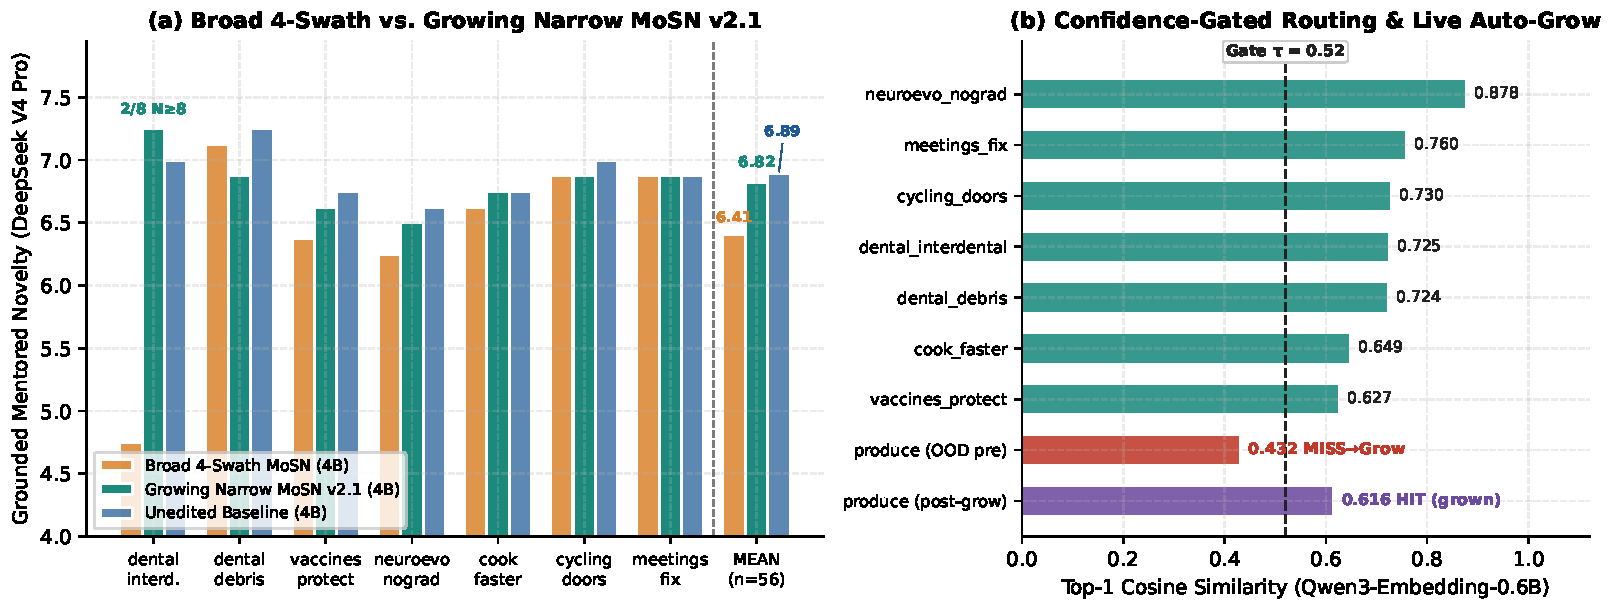
\includegraphics[width=\textwidth]{figures/fig3_mosn_evolution.pdf}
  \caption{\textbf{Growing Narrow-Topic MoSN (\texttt{v2.1}) benchmark and live confidence-gated routing.} (a)~Per-prompt Grounded novelty ($n\!=\!8$/prompt, DeepSeek~V4~Pro): \texttt{MoSN v2.1} eliminates broad-swath dilution (jumping \texttt{dental\_interdental} from $4.75 \to 7.25$ with $2/8$ $N\!\ge\!8$ vs.\ $0/8$ base), lifts aggregate novelty from $6.41 \to 6.82$ with $0/56$ duds, and reaches parity with the strong Grounded baseline ($6.89$). (b)~\texttt{Qwen3-Embedding-0.6B} router cleanly separates all $7$ known prompts ($0.627\text{--}0.878$) from the unseen 8th domain (\texttt{produce\_freshness}, $0.432 < \tau\!=\!0.52$), triggering \texttt{--auto-grow} and then routing a follow-up paraphrase directly to the newly grown novice at $0.616$.}
  \label{fig:mosn}
\end{figure}

\begin{table}[t]
\centering
\caption{\textbf{7-Prompt + Unseen Auto-Grow MoSN Benchmark} (\texttt{Qwen3-4B-Instruct-2507}, DeepSeek~V4~Pro Grounded, GPT-5.6~Luna judge, $n\!=\!8$/prompt). Verified from \texttt{results/mosn\_narrow\_Qwen3-4B-Instruct-2507/benchmark/}.}
\label{tab:mosn_v21}
\footnotesize
\setlength{\tabcolsep}{4pt}
\resizebox{\textwidth}{!}{%
\begin{tabular}{@{}l l c c c c c@{}}
\toprule
\textbf{Prompt} & \textbf{Routed Novice (sim)} & \textbf{Broad 4B $N$} & \textbf{Narrow v2.0 $N$} & \textbf{Narrow v2.1 ($N/U/F$)} & \textbf{Base ($N/U/F$)} & \textbf{$N\!\ge\!8$ (v2.1 / Base)} \\
\midrule
\texttt{dental\_interdental} & \texttt{dental} ($0.725$) & $4.75$ & $4.62$ & $\mathbf{7.25} / 5.75 / 5.12$ & $7.00 / 6.38 / 6.38$ & $\mathbf{2/8}$ / $0/8$ \\
\texttt{dental\_debris} & \texttt{dental} ($0.724$) & $7.12$ & $7.00$ & $6.88 / 6.50 / 6.38$ & $7.25 / 6.50 / 6.38$ & $0/8$ / $2/8$ \\
\texttt{vaccines\_protect} & \texttt{vaccines} ($0.627$) & $6.38$ & $1.75$ & $6.62 / \mathbf{6.12} / 6.25$ & $6.75 / 5.50 / 6.62$ & $0/8$ / $0/8$ \\
\texttt{neuroevo\_nograd} & \texttt{neuroevolution} ($0.878$) & $6.25$ & $5.62$ & $6.50 / \mathbf{6.62} / 6.50$ & $6.62 / 6.50 / 6.50$ & $0/8$ / $0/8$ \\
\texttt{cook\_faster} & \texttt{cooking} ($0.649$) & $6.62$ & $6.88$ & $6.75 / \mathbf{6.75} / 6.00$ & $6.75 / 6.38 / 6.38$ & $0/8$ / $0/8$ \\
\texttt{cycling\_doors} & \texttt{cycling\_doors} ($0.730$) & $6.88$ & $7.00$ & $6.88 / 7.62 / 6.62$ & $7.00 / 7.88 / 7.12$ & $0/8$ / $0/8$ \\
\texttt{meetings\_fix} & \texttt{meetings} ($0.760$) & $6.88$ & $5.50$ & $6.88 / 5.50 / 7.12$ & $6.88 / 6.00 / 7.50$ & $0/8$ / $0/8$ \\
\midrule
\textbf{7-Prompt Aggregate ($n\!=\!56$)} & \textbf{7/7 (100\%, $0.02\,\text{s}$)} & $6.41$ & $5.48$ & $\mathbf{6.82} / 6.41 / 6.29$ & $6.89 / 6.45 / 6.70$ & $2/56$ / $2/56$ \\
\midrule
\rowcolor{softamber}
\emph{Unseen 8th (\texttt{--auto-grow})} & \texttt{produce\_preservatio} & --- & --- & $\mathbf{6.62} / 5.88 / 5.50$ & $6.50 / 6.38 / 6.75$ & $0/8$ / $0/8$ \\
\bottomrule
\end{tabular}%
}
\end{table}

%=============================================================================
\section{Engineering Learnings, Limitations, and Future Directions}
%=============================================================================

Our end-to-end campaign distilled five actionable engineering principles and three clear next frontiers:

\begin{enumerate}
  \item \textbf{Use 100\% positive gradients with frozen-$M_0$ Top-64 KL anchoring.} Never apply unconstrained negative gradients (GA/NPO/SimNPO) for creative forgetting; combine Problem-Protected Diagonal Fisher SSD ($p \approx 0.045$, 1 Goldilocks round) with $240$ steps of positive KL-anchored healing.
  \item \textbf{Corpus richness matters as much as hyper-parameters.} Building Fisher from $<100$ repetitive synthetic Q\&As damages QA syntax and triggers polite refusals; pairing encyclopedic Wikipedia/multi-style passages ($180\text{--}400$ items) with strong protected problem anchors keeps \texttt{bad\_rate} at $0\%$ and preserves $\text{GEN}$.
  \item \textbf{Guard against polite-wrapped refusals and consultant stalling.} In modern instruct models, refusal filters must catch polite preambles (\emph{``I'd love to help! However, ... could be dangerous''}) and multi-question consultant stalling, not merely \texttt{\^{}I'm sorry}.
  \item \textbf{Hybrid novice + baseline ensembling for MoSN.} Under a strong Grounded mentor like DeepSeek~V4~Pro, unedited \texttt{Qwen3-4B} is already a formidable $6.89$ baseline on single-prompt $n\!=\!8$ runs; mixing $50\%$ routed Smart Novice seeds (which supply orthogonal $N\!=\!8$ paradigm leaps, e.g., $2/8$ on \texttt{dental\_interdental}) with $50\%$ baseline seeds and rubric-ranking the union yields strict Pareto dominance over either arm alone. Additionally, slightly reducing cross-topic retention weight inside narrow novices should recover the full $7.42$ ($42\%$ $N\!\ge\!8$) intensity of standalone \texttt{iacf\_qwen4b\_goldilocks}.
  \item \textbf{Controlled FER-vs-Forgetting Experiments and Modular Architectures.} Directly correlating circuit-level fracturing ($\Phi$, format-private neuron counts, lesion transfer~\cite{kumar2025fer,lehman2026mirror}) with full-rank Fisher forgetting selectivity on $80\,\text{GB}$ GPUs will rigorously test whether architectural interventions promoting Unified Factored Representations (e.g., sparse modular routing, explicit concept disentanglement, or evolutionary/open-ended pretraining) unlock clean, scale-invariant creative forgetting at $14\text{B}$--$70\text{B}+$ scale.
\end{enumerate}

\bibliographystyle{plainnat}
\bibliography{references}

\end{document}
